\documentclass{article} 
\usepackage[estonian]{babel}
%\usepackage{fontspec} 
\usepackage{graphicx}
\usepackage{hyperref}
\usepackage{natbib}
\usepackage{booktabs}
\usepackage{makeidx}
\usepackage{tgpagella}
\usepackage[T1]{fontenc}

\hypersetup{
    colorlinks=true,       % false: boxed links; true: colored links
    linkcolor=black,          % color of internal links
    citecolor=black,        % color of links to bibliography
    filecolor=magenta,      % color of file links
    urlcolor=black           % color of external links
}

\renewcommand\refname{Viited}

\makeatletter 
\def\s@btitle{\relax} 
\def\subtitle#1{\gdef\s@btitle{#1}} 
\def\@maketitle{% 
  \newpage 
  \null 
  \vskip 2em% 
  \begin{center}% 
  \let \footnote \thanks 
    {\LARGE \@title \par}% 
                \if\s@btitle\relax 
                \else\typeout{[subtitle]}% 
                        \vskip .5pc 
                        \begin{large}% 
                                \textsl{\s@btitle}% 
                                \par 
                        \end{large}% 
                \fi 
    \vskip 1.5em% 
    {\large 
      \lineskip .5em% 
      \begin{tabular}[t]{c}% 
        \@author 
      \end{tabular}\par}% 
    \vskip 1em% 
    {\large \@date}% \\
    \vfill
  \end{center}% 
  \par 
  \vskip 1.5em} 
\makeatother 


\title{IFI7013. IT Strateegiline Juhtimine}
\subtitle{Märkmed ja kommentaarid}
\date{\today}
\author{Andres Kütt}
%\institute{Riigi Infosüsteemi Amet}

\newcounter{slidenum}
\setcounter{slidenum}{2} % set to 2 if want to exclude title page of presentation

\newcommand\showslide{
%  \clearpage 
  \begin{center}
    \framebox{\includegraphics[page=\arabic{slidenum},width=.99\textwidth]{esimene_kontakt_beamer.pdf}}
%	\includegraphics[page=\arabic{slidenum},width=.65\textwidth]{esimene_kontakt_beamer.pdf}
    \stepcounter{slidenum}
  \end{center}
  \clearpage
}

\begin{document}
\maketitle
\clearpage
\tableofcontents
\clearpage

\section{Arhitektuur}
\subsection{Printsiipidest}
Arhitektuuriga süvitsi tegelemisel on hea mõte pidada printsiipide päevikut. Arhitektuuris on mõttemudelil oluline koht ja seega on mõistlik tegeleda oma isikliku mõttemudeli arendamise ning dokumenteerimisega. Printsiibipäevik on üks viis seda teha. Printsiip on miski, mis tundub kehtivat alati ning mis ei sõltu teistest. Teatavas mõttes on tegemist universaalse tõega. Üheks näiteks printsiipidest arvutivõrkude vallas on \cite{callon1996rfc}. Printsiibipäeviku mõte on selles, et iga kord, kui igapäevases töös tundub mõni printsiip silma jäävat, kirjutatakse see jalamaid üles. Perioodiliselt vaadatakse päevik üle lootuses destilleerida kirja pandust veel universaalsemaid ja üldisemaid põhimõtteid. Üks näide sellisest päevikust on \cite{archprinciples}. 

\section{Tarkvaratehnika}
\subsection{Kood ei roosteta. Või siiski?}
Joel Spolsky ütleb, et reeglina on väga halb mõte oma koodibaasi ümber kirjutada, sest kood ju "ei roosteta" \citep{joelrust}. Ta toob mitu näidet väga ebameeldivate tagajärgedega ümber-kirjutamis ettevõtmiste kohta ning, tõesti, neid on ka siinkirjutaja praktikas mitmeid ette tulnud. Põhjuseid on mitmeid, peamiseks ehk paratamatu teadmuskadu: iga tükki koodi on juba enne rakenduse valmimist kümneid kui mitte sadu kordi muudetud ja parandatud parandamaks vigu, ületamaks nõuete ebatäielikkust jne. Nii kaob igasugune võimalus hinnata, kas kood on selline, nagu ta on, põhjusega või põhjuseta. Rääkimata analüüsist, kas põhjus jätkuvalt kehtib. Miks siis tekib vahel siiski kohu asju ümber teha ning miks on Eestis kehtestatud \emph{no legacy policy}?

Ühest küljest on asja taga kindlasti programmeerijad. Nagu Spolsky õigesti osundab, on koodi lugemine palju keerulisem, kui selle kirjutamine. Seega, eriti kui tegu on kellegi teise koodiga, on programmeerijale oluliselt lihtsam kirjutada uus kood kui üritada vanast aru saada. Loomulikult tõlgitakse vahe rahanumbriks ning uue süsteemi ehitamine võib vana turgutamisest oluliselt odavam näida. Erinevalt uue süsteemi ehitamisest, ei ole vana muutmine kergesti hinnatav ning tellija ees on kas väike fikseeritud number ebamäärase kahjuga või suur riskantne number ebamäärase tuluga. 

Teisalt võib ümberkirjutamissoovi taga olla lihtne äriliste riskide vähendamine. Vana kood peidab endas alati üllatusi ning riskide vähendamiseks võib pakkuja eelistada uue kirjutamist. 

Mõlemal juhul tekib lihtsasti olukord, kus tellijal ja otsuse tegijal ei ole piisavalt tehnilist teadmist ja/või informatsiooni vana süsteemi kohta. Erinevalt koodist teadmus kindlasti kõduneb. Sel puhul on mõistlik käivitada väikesemahuline konkreetsete tulemustega piloot rakenduse kvaliteedi hindamiseks. Selle lõppedes on nii tellijal kui täitjal palju selgem ülevaade, kui keeruline vana koodibaasi putitamine tegelikult on.

Olemasoleva koodi puhul võib tegu olla ka "pusaga": süsteemiga, mis on aja jooksul kas arhitektuuriliselt või tehnoloogiliselt keeruliseks kasvanud. Nii arhitektuuri kui tehnoloogia puhul on kindlasti tegu ka mööduva moega, tehno\-loogiad ning arhitektuurimustrid vananevad. Samas ei ole kindlasti tegu \textit{carte blanche} põhjusega rakendusi ümber kirjutada, COBOLi süsteeme on edukalt veebirakendustega integreeritud. Jällegi on mõistlik läbi viia piloot ning teha otsus kindla teadmise, mitte kellegi arvamuse pinnalt.

\begin{figure}[htp]
	\begin{center}
		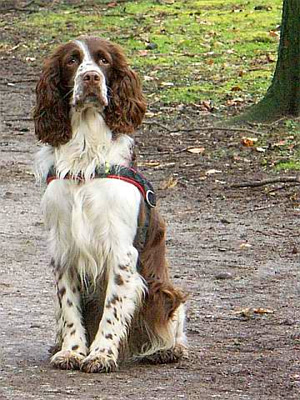
\includegraphics[height=4cm]{spaniel.jpg}
\includegraphics[height=4cm]{wolf.jpg}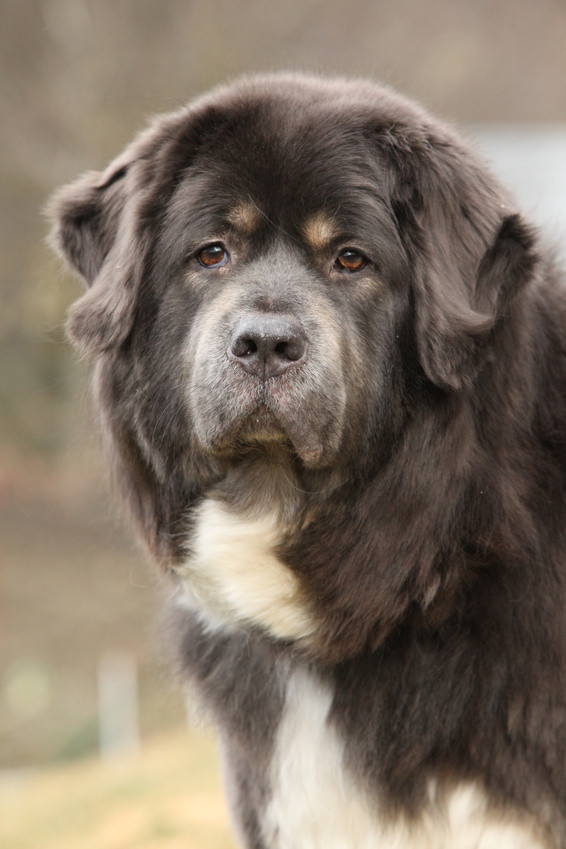
\includegraphics[height=4cm]{mastiff.jpg}
		\caption{Spanjel, hunt ja mastif}
	\end{center}
\end{figure}

Niisiis, koodi ümber kirjutamine on kallis, keeruline ning seotud oluliste riskidega. Samas on olemasoleva rakenduse putitamisel samuti üks oluline puudus: me toimime jätkuvalt kord juba defineeritud arhitektuuri, täpsemalt öeldes kontseptsiooni, raamides. Ehk, asjade ümber kirjutamine annab võimaluse innovatsiooniks ning asjade puhtalt lehelt uuesti mõtestamiseks. Jah, spanjelist on ilmselt võimalik mastifi-laadne elukas aretada aga võibolla on efektiivsem alustada siiski nende ühisest eellasest, hundist? Kindlasti tuleks keskenduda mitte tehnilisele vaid ärilisele innovatsioonile ümber mõtestades äriprotsesse, automatiseerides ning efektiivistades. Seejuures on muidugi eelduseks, et meil on piisavalt aega ja raha seda mõttetööd põhjalikult ette võtta ning et on alust eeldada, et tulemus praegusest olukorrast oluliselt erineb.

Lõpuks tuleb panna kõrvuti süsteemi ümber kirjutamise kulu (korrutades esiaglse hinnangu vähemalt kahega), olemasoleva muutmise ning mõlema alternatiivi halduskulude nüüdisväärtus. Kui nüüd tundub, et rakenduse uuesti kirjutamine on siiski mõistlik, on oluline aru saada, miks nii läks. Jällegi Joelile toetudes, ei ole mõistlik eeldada, et kui ühel korral ei õnnestunud hankida mõistlikku süsteemi või seda pusaks muutumast hoida, siis teisel korral asjad teisiti lähevad. On oluline, et suudetakse välja tuua konkreetsed tegevused, mille abil hoidutakse vajadusest süsteem uuesti ümber kirjutada. Siinkohal kuuleb ilmselt argumenti \emph{build one to throw away} aga sel juhul peaks olema võimalik vähemalt üles kirjutada, mida esimesest korrast täpselt õpiti.

\subsection{Tehniline võlg}
On kriitiline, et tellija saaks aru oma tegevuse tagajärgedest. Mis, arvestades teo ja selle tagajärje ajalist vahet, on väga keeruline. Põhjus on selles, et tehnilise võla likvideerimine tuleb arenduse läbilaskevõime arvelt. Järelikult tähendab tehnilise võla kuhjumine, et arenduse läbilaskevõime ajas kahaneb. Kui tellija ei saa aru, et tema otsus tekitas tehnilise võla, on IT-juhil kaks põhimõttelist otsust. Ta kas keeldub tehnilist võlga tekitamast, näib paindumatu ja lastakse lahti või ta võtab tehnilise võla, asub seda IT võimekust vähendades likvideerima ning ta lastakse lahti. Ehk, häid valikuid ei ole. Järelikult ei ole IT juhil muud valikut peale tellija harimise.

\section{IT valitsemine}
\subsection{Poliitikavastasus. Hundid ja jänesed}
Kujutlegem lihtsat ökosüsteemi, mis koosneb huntidest ja jänestest. Hundid söövad jäneseid, jänesed elavad õhust ja armastusest (mida mõlemat on piisavalt). Oletagem, et meil on soov tõsta huntide arvukust. Seepärast tuuakse mujalt ja lastakse metsa lahti viis emast ja viis isast hunti. Mis juhtub? 
\begin{itemize}
	\item Huntide arvukus tõuseb kümne lisandunud hundi võrra
	\item Kuna kümme lisandunud hunti tahavad süüa, siis väheneb jäneste arvukus. Ajaühikus ära söödavate jäneste hulk ju suureneb
	\item Kuna jäneseid on vähem, väheneb ka jäneste juurdekasvu kiirus. Ära söödud jänesed ju uusi jäneseid ei tee. Samuti tahavad uued hundid ka homme süüa
	\item Seega hakkab jäneste arvukus vähenema
	\item Misjärel hakkavad hundid nälga jääma, sest kõigile enam jäneseid ei jagu
	\item Mistõttu saavad hundid vähem järglasi ja langeb nende juurdekasvu kiirus
	\item Kuna hundid surevad vanadusse ikka sama tempoga, hakkab huntide arvukus vähenema
	\item Kui huntide arvukus on jõudnud esialgsele tasemele, on kõigile jälle piisavalt jäneseid 
\end{itemize}

Nii taastub esialgne olukord, algne huntide lisamine ei ole andnud soovitud tulemust. Huntide arvukus võiks tõusta hoopis tõstes jäneselaste arvu jäneseperekonnas ehk nende juurdekasvu kiiruse tõstmisega. 

\subsection{Inimeste valitsemine}
Valitsemise üsna lahutamatu osa on paraku vajadus inimesed organisatsioonist eemaldada. Jättes kõrvale juriidilised ja muud nüansid, on oluline aru saada, et mõtteliidri (\emph{thought leader}) lahkumine on meeskonna dünaamika jaoks oluline sündmus. Samuti on oluline mõista, et tegu on vältimatu protsessiga, mis seega on mõistlik läbi viia kontrollitult ja minimaalsete kadudega. Järgnevas selleks mõned näpunäited: 

\begin{itemize}
	\item Vii inimene organisatsioonist välja enne, kui tema vastuolud muutuvad meeskonna vastuoluks. Definistiooni järgi inimesed järgnevad liidrile ning kui tollel on kellegagi vastuolud, kanduvad nood paratamatult varem või hiljem meeskonda. Kui hiljaks jääda lahkuvad (või tuleb vastuseisu tõttu eemaldada) ka teised tiimi liikmed peale juhi. Nii võib oskamatu käitumisega vallandada lumepalliefekti, mis organisatsiooni kiiresti ajudest tühjendab.
	\item Väike (!) hulk võtmeisikuid peab plaanist ette teadma, sealhulgas muidugi ka eemaldatav ise. Nii on neil ühest küljest võimalik tulevaseks kriisiks valmistuda kuid teisalt saab nii vältida emotsionaalset avalikku käitumist ning muidu üllatusi. Etteteatamisaeg võib ulatuda mõnest päevast mõne tunnini. Pikem aeg tekitab permanentse kriisi olukorra ja kommunikatsioon väljub kontrolli alt
	\item Kommunikatsiooni kolm sammu. Kõik sammud läbitakse väga lühikeste (kõige rohkem mõned tunnid) intervallidega vältimaks uudiste lekkimist (ingl. \emph{techcrunch meltdown} tuntud tehnoloogiauudiste portalli järgi) ning minimeerimaks kriisi kestvust. 
		\begin{enumerate}
			\item "Vanaisa"\footnote{Juhi juht. Selles kontekstis isik, kes teeb otsuse inimene välja viia.} teade. Nii antakse teada, kes olukorda kontrollib. Sisaldab
				\begin{itemize}
					\item Kes lahkub millal ja miks. Tekst olgu viisakas, inimesed kas teavad niigi või suudavad ridade vahelt lugeda
					\item Mis juhtub järgmisena ja millal. Inimestele ei meeldi ebakindlus, hirmud tuleb maha võtta. Oluline punkt siin: kes ja millal asendab lahkuja?
					\item Muutused organisatsiooni toimimises. Lahkuja oli kindlasti osaline mingites äriprotsessides (koodi ülevaatused, tarnete vastu võtmine jms.), kuidas need edasi toimima hakkavad?
				\end{itemize}
			\item Lahkuja teade. Tavaliselt suunatud lähematele kolleegidele. Võib olla suhteliselt otsekohene aga kui on karta midagi mürgist, võib (viisakalt) paluda teksti kooskõlastamist
			\item Avalik teade. Kui vähegi usutav, võiks tekst olla kiitvas, positiivses ja tänulikus toonis. Kui mitte, siis lakooniline kuiv tekst.
		\end{enumerate}
\end{itemize}

\subsection{Ressursijuhtimine}
Järgnev on üks võimalik vaade asjadele: selgesti on avaliku- ja erasektori suhtumine rahasse erinev. Ainus põhjus, miks maksumaksja riigile raha annab, on, et selle raha eest osutataks avalikku teenust. Kui nüüd riik korjab raha kokku, kuid selle eest mõistlikku avalikku teenust ei osuta (ka reservide kogumine on avalik teenus), siis on tegu maksumaksja asjatu koormamisega. Erasektoris jaotatakse kasum omanike vahel, riigis selle mehhanismi ekvivalenti ei eksisteeri. Järelikult on erasektoris pigem surve raha mitte kulutada samas kui riigisektoris on pigem surve raha eest võimalikult palju teenust osutada.  

\subsection{Protsesside juhtimine}
\subsubsection{Organisatsiooni kiirendamine}
Suurepärane näide organisatsiooni kiirendamisest on Singapur. Joonisel \ref{fig:kasv} on toodud viie riigi GNI aastatel 1995 kuni 2012. On näha, kuidas USA, Eesti, Läti ja Vene Föderatsioon kasvavavad suuresti samas rütmis, kuigi absoluutnumbrites on USA teistest kaugel ees. Singapur aga on suutnud aastast 2002 näidata teistest oluliselt kiiremat kasvu. Isegi arvestades 2008. aasta kriisi mõju, on kasv teistest oluliselt kiirem. Lühike järeldus joonisest on, et ühel või teisel viisil on Singapur suutnud mitte ainult kasvada, vaid kasvada teistest kiiremini. Kui Eesti aga ka jätkab senist stabiilset kasvu, ei õnnestu meil ilmselt kunagi USAle järele jõuda. 

\begin{figure}[h]
	\begin{center}
		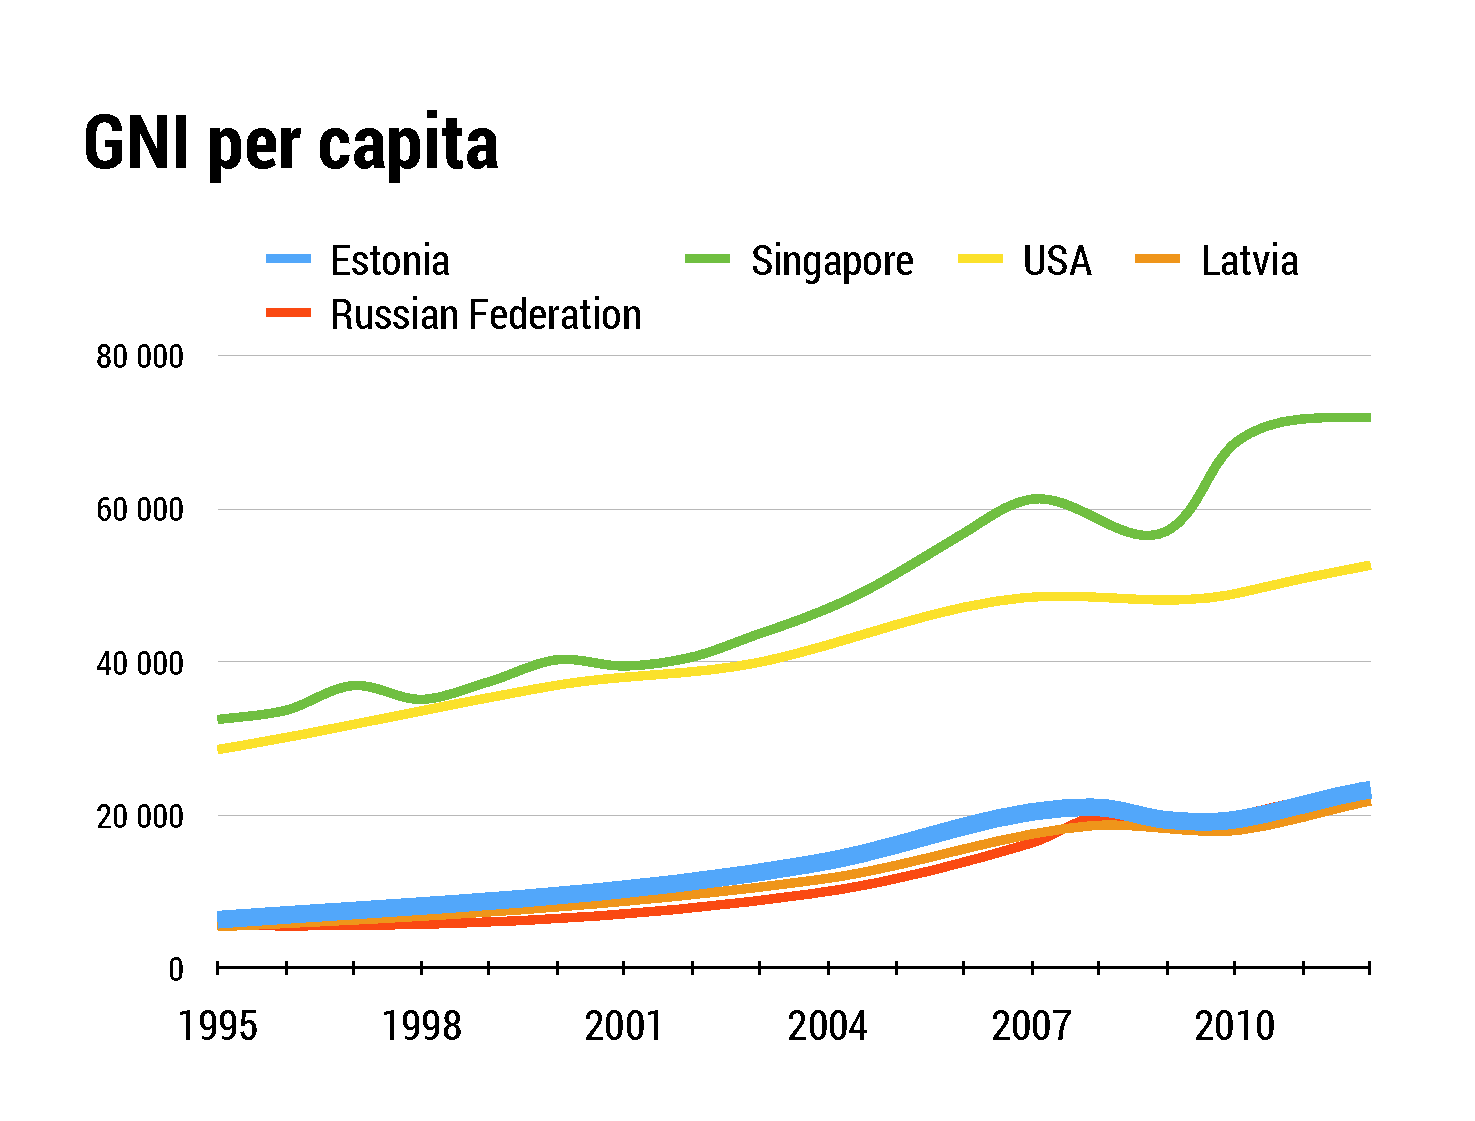
\includegraphics[width=\textwidth]{kasv.pdf}
		\caption{Riikide GNI võrdlus. Maailmapanga andmed.}
		\label{fig:kasv}
	\end{center}
\end{figure}


\section{Jätkusuutlik areng}
\subsection{Konteksti kaardistamine}
Väärtusahel on ikka olnud üheks viisiks ärimudelit visualiseerida ja sellest mõelda. Tegu on siiski ka makrotasandil üllatavalt kasuliku vahendiga keeruliste suhtevõrgustike analüüsimiseks. Meetod on lõtv ja vabalt kohaldatav, kuid laias laastus saab talle siiski struktuuri anda. Kontekstikaardistus käib nii. 

Grupp inimesi viib valge tahvliga ruumis läbi järgmised sammud:
\begin{enumerate}
	\item Joonistame üles kõik huvitatud osapooled. Rahulikult võib ignoreerida osapoolte tüüpe ja omavahelisi hierarhilisi sõltuvusi\footnote{Keerukamatel juhtudel võib need eraldi, näiteks teise värviga, välja tuua}. Samal pildil võivad eraldi kehad olla töötaja ja tööandja. 
	\item Lähtudes meid kõige enam huvitavast (tavaliselt konkreetse kokkusaamise algataja ning kasusaaja), küsime iga osapoolte paari kohta
		\begin{itemize}
			\item Mida saab osapool A osapoolelt B?
			\item Mida saab osapool B osapoolelt A?
		\end{itemize}
	\item Kõik seosed joonistame üles õiges suunas näitavate nooltega 
	\item Valideerime pildi küsides iga osapoole kohta: "kust na saavad seda, mida nad ära annavad?"
	\item Analüüsime pilti. Näiteks on oluline tuvastada "väravavahid" ehk kahte omavahel tihedalt seotud ökosüsteemi ühendavad graafi tipud
\end{enumerate}

\begin{figure}[h]
	\begin{center}
		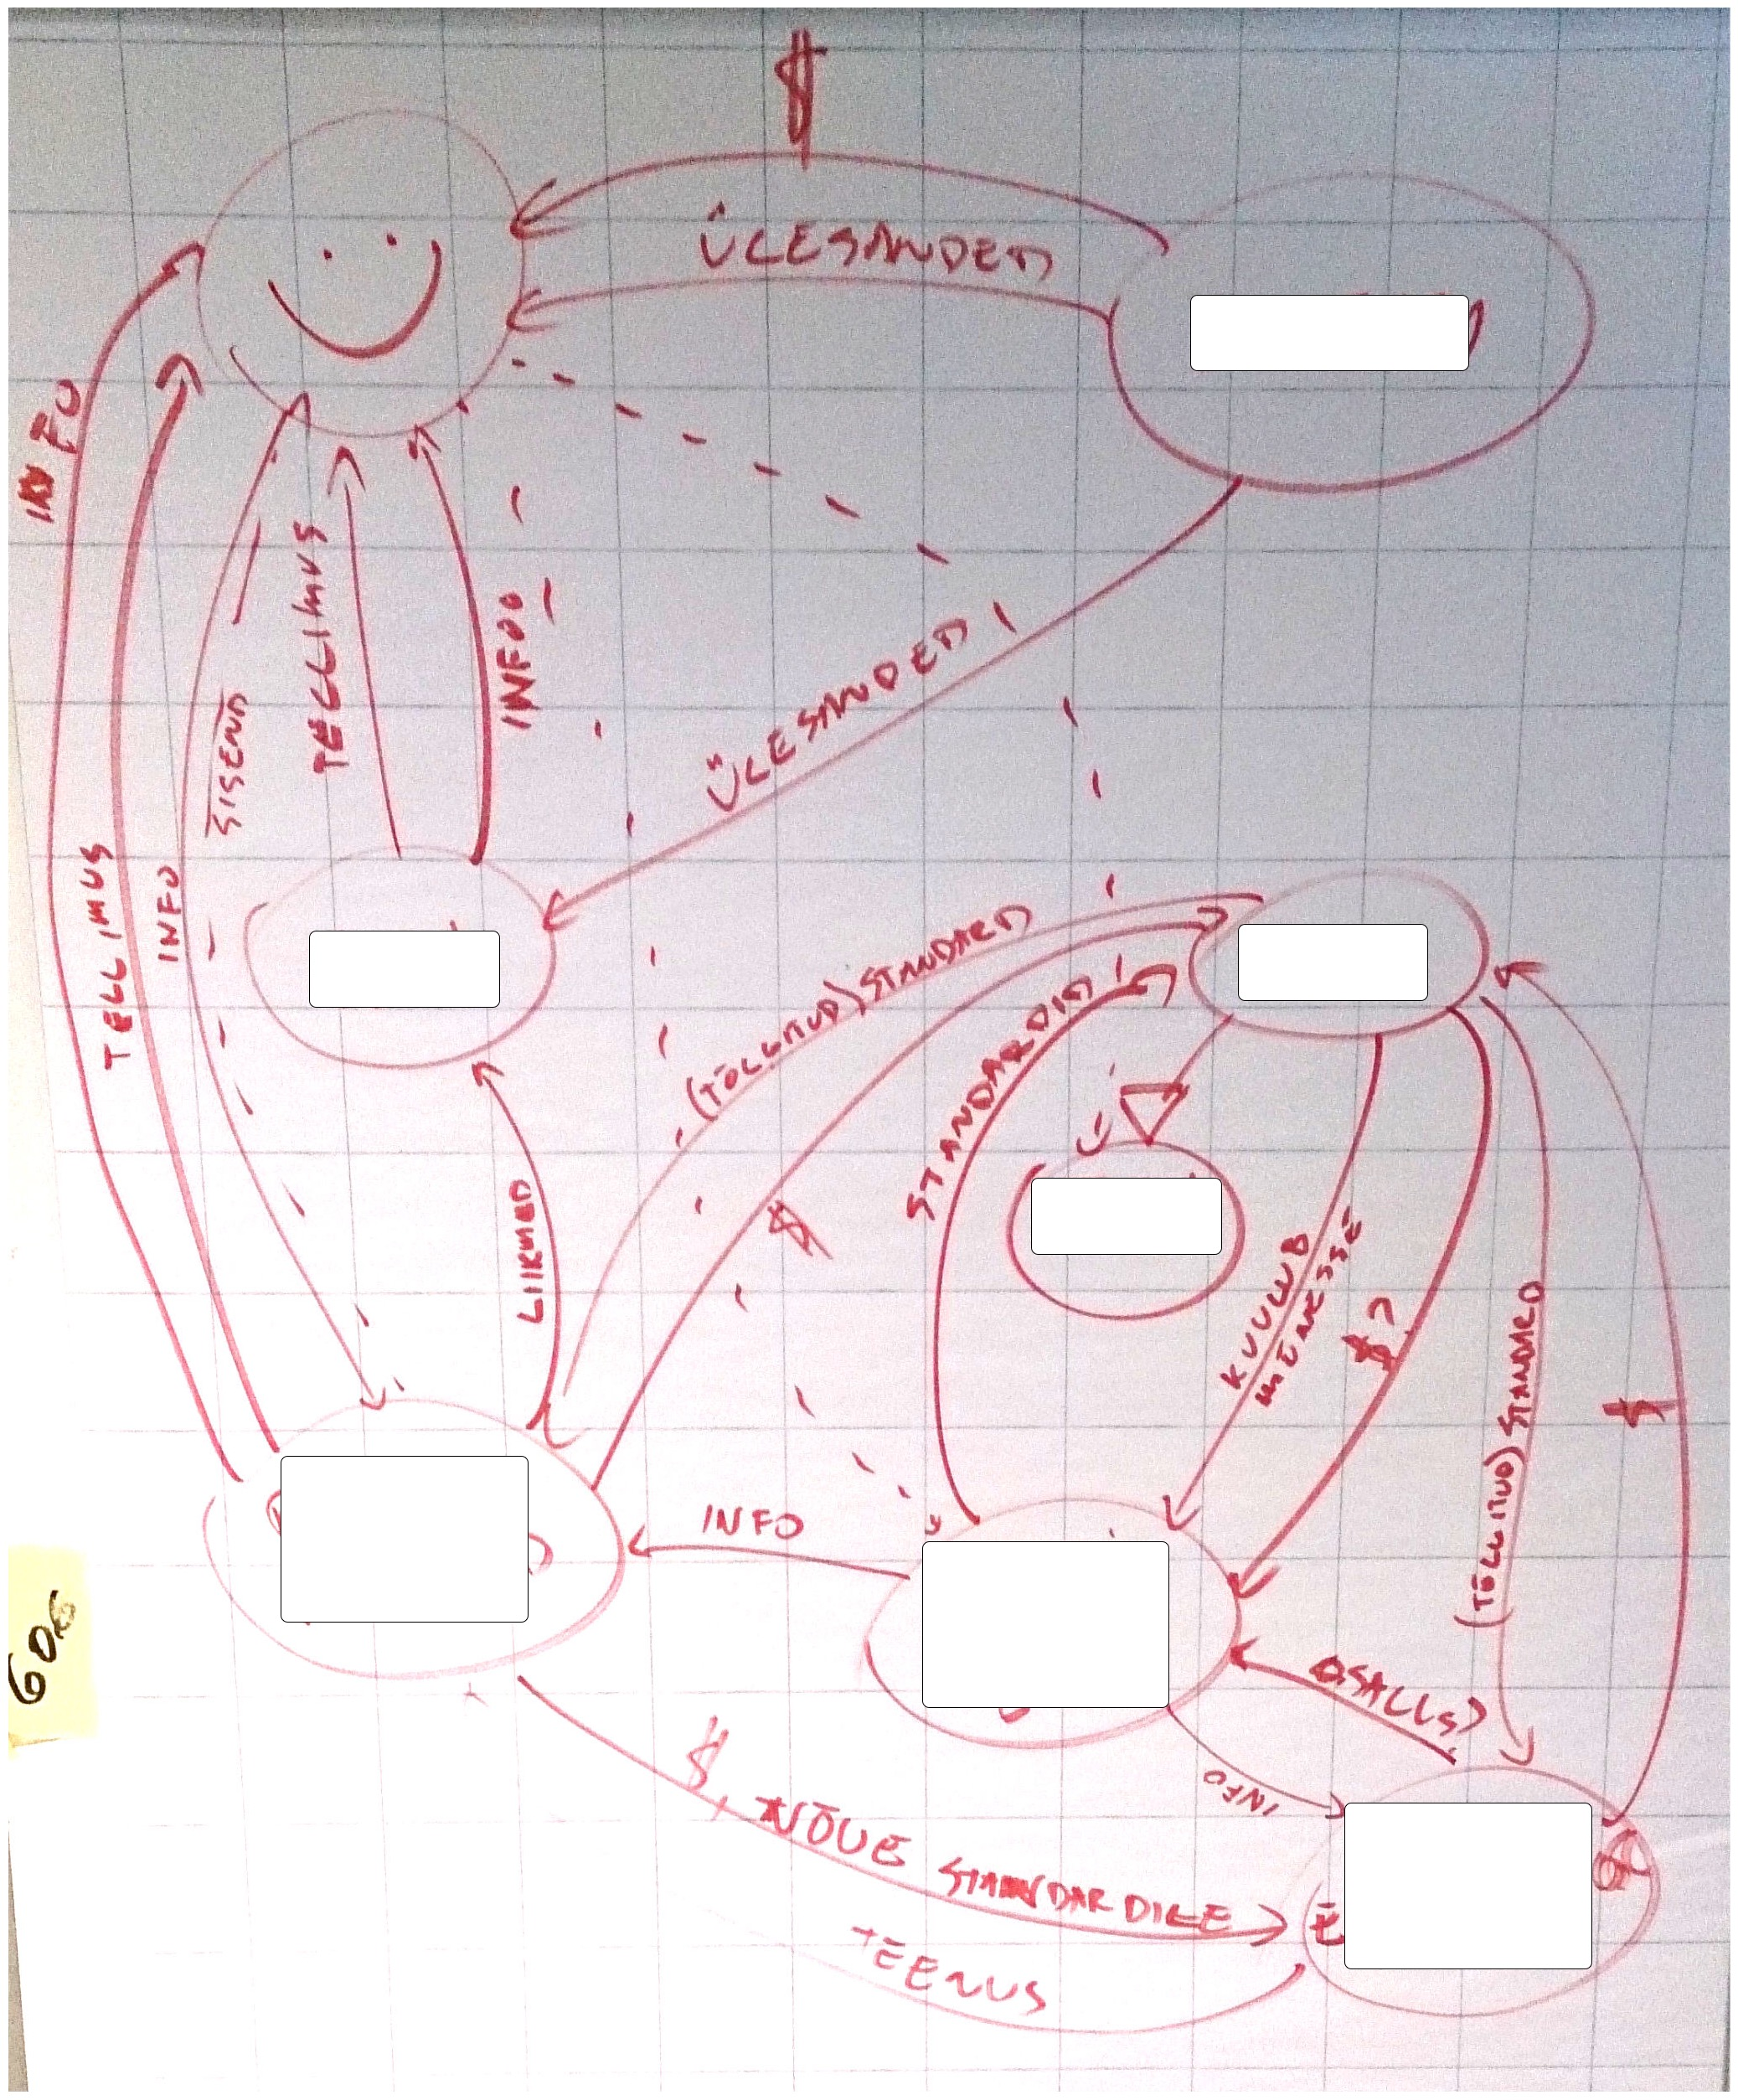
\includegraphics[width=.7\textwidth]{seosed.jpg}
		\caption{Näide seoste diagrammist}
		\label{fig:seosed}
	\end{center}
\end{figure}


\subsection{Piiridest ja nende ületamisest}
Eelmise sajandi seitsmekümnendatel töötas Jay Forrester Rooma Klubi tellimusel välja mudeli maailma rahvastiku kasvu uurimiseks. Forresteri õpilased on mudelit hiljem täiendanud, hetkel on ehk parim lugemismaterial \cite{meadows1992beyond}. Ennustused ei ole roosilised, pigem vastupidi. Ühe tõenäolise võimalusena nähakse ette, et rahavastik ületab suurelt piirid, mida tehnoloogia võimaldab planeedil Maa ära toita ning mahutada ja et järgneb mõõdukas kollaps. Rahvastik kahaneb kiiresti ning palju ning toimub tugev konkurents ressursside pärast (sest kõigile lihtsalt ei jätku). 

\section{Riskijuhtimine}
\subsection{Paradigmamuutus}
Riskijuhtimise paradigmamuutust tingivad järgmised trendid:
	\begin{itemize}
		\item BCP\footnote{\emph{Business Continuity Plan}} keerukus/hind kasvab eksponendina süsteemi keerukusest
			\begin{itemize}
		\item Facebookil ei ole kuskil teist andmekeskust igaks juhuks jõude seismas. See oleks liiga kallis
		\item Väliste partnerite puhul ei ole alati võimalik alternatiivi leida
		\item Äriprotsesside toimimisele ei ole vahel enam mitte-elektroonilist alternatiivi
	\end{itemize}

		\item BCP efektiivsus kahaneb eksponendina süsteemi keerukusest
			\begin{itemize}
		\item Kuidas taastub pilveteenusepakkuja täielikust andmekaost?
		\item Keerulist süsteemi ei pruugi õnnestuda ka mitte ajuti taastada, kui palju ka ei kulutaks. Kui Skype p2p võrk päriselt maha kukub, seda sisuliselt ei olnud võimalik taastada
		\item Äriplaanid, kliendiandmed, ideed, dokumentatsioon on üha enam immateriaalne ja seega kergesti teisaldatav
	\end{itemize}

		\item Üksikute riskisündmuste asemel peame rääkima pidevast, kasvavast ja kuju muutvast survest
			\begin{itemize}
		\item Ka kuritegevuses on edukas see, kes suudab oma ärimudeli võimalikult efektiivselt võimalikult suureks skaleerida
		\item Keerulises süsteemis on väga palju elemente ja nende interaktsioone, mõne katki mineku tõenäosus on suur
		\item Inimese kognitiivset võimet ületavate süsteemide puhul kasvab kiiresti operaatori vigade tõenäosus. Mistõttu ma olen suhteliselt ettevaatlik Eesti Vabariigi infosüsteemi torkimisega
	\end{itemize}

		\item Riskifaktoreid ei saa enam suruda aktsepteeritavale tasemele
			\begin{itemize}
		\item Riik suudab tagada, et tänaval ei jookse nagaaniga vehkiv jõuk, internetis ei ole see võimalik
		\item Süsteemi kõik elemendid ei ole kontrolli all. Vt. esimese kontakti slaidid Yosemite intsidendist
		\item Kuna info liigub, kerkib kiiresti esile uusi (Google: \emph{"ATM gas attacks"})
		\item Turvalist ega vigadeta tarkvara ei ole reaalne toota. Heartbleed istus aastaid laialt kasutatud open source tarkvarateegis kõigi silmade all
	\end{itemize}

\end{itemize}
\subsection{Süsteemiohutuse vaatenurk}
Eelnevalt loetletu kõrvale seab \cite{leveson2011engineering} oma nimekirja asjaoludest, mis sunnivad loobuma senistest süsteemide ohutust käsitlevatest mudelitest:
\begin{itemize}
	\item Kiire tehnoloogiline muutus
	\item Vähenev õppmisvõimekus, mida põhjustab järjest lühenev toote elutsükkel
	\item Õnnetuste iseloom on muutumas, eriti tänu tarkvara tihedasse integreerumisse igapäevaellu
	\item Uued ohtude tüübid. Nanotehnoloogia, keemia, antibiootikumid jne.
	\item Suurenev keerukus ja seotus
	\item Vähenev tolerants üksik-õnnetuste suhtes, mis tuleneb süsteemide suurusest ning meie suurenevast sõltuvusest tehnoloogiast
	\item Prioriteetide seadmise ja valikute tegemise keerukus
	\item Inimeste ja automaatide järjest keerulisemad suhted
	\item Muutuv regulatiivne ja avalikkuse vaade ohutusele. Üksikindiviid ei ole enam suuteline oma vahetu keskkonna ohutust kontrollima
\end{itemize}

\subsection{Kaos ja ahvid}
Üks suurimaid probleeme slaididel ja loengus kirjeldatud paradigmamuutusega toime tulekul on inimeste hoiakud. Kui ühe serveri puhul võis loota, et see niipea katki ei lähe ja kui läheb, siis on teine varuks, siis 1000 serveri puhul läheb iga päev mõni katki. Sama lugu on küberrünnetega. Inimeste mõttemudel muutub aga aeglaselt. Probleemi on huvitavalt lahendanud Netflix \citep{monkey}. Nende vahend lihtsalt käib ja lülitab servereid välja, kõik teavad seda. Ehk, iga teenus peab olema suuteline sellist käitumist taluma. Sisuliselt on Netflix teadmata parameetritega rikete mürafooni asendanud palju tugevama kuid tuntud parameetritega signaaliga.   

%\showslide
%\showslide
%\lipsum[1-5]

%\showslide
%\lipsum[2]
\nocite{*}
\bibliographystyle{plainnat}
\bibliography{it_strateegia} 

\end{document}
